\begin{figure}[htbp]
\centering
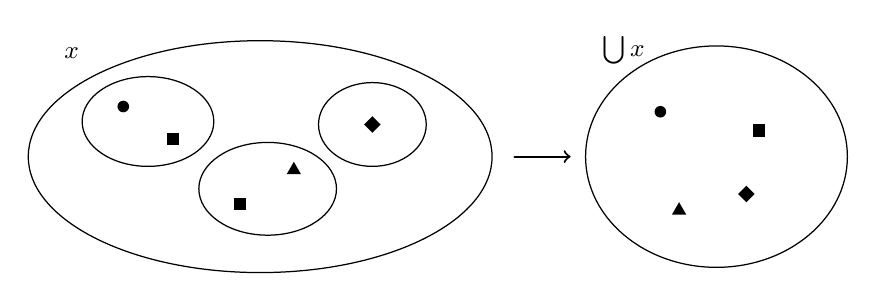
\begin{tikzpicture}[
    scale=0.95,
    line cap=round,
    every node/.style={font=\small},
    conjunto/.style={draw, line width=0.45pt},
    seta/.style={->, line width=0.75pt},
    pics/ponto/.style={
        code={
            \fill (0,0) circle[radius=2.1pt];
        }
    },
    pics/quadrado/.style={
        code={
            \fill (-2.2pt,-2.2pt) rectangle (2.2pt,2.2pt);
        }
    },
    pics/triangulo/.style={
        code={
            \fill (90:3pt) -- (210:3pt) -- (330:3pt) -- cycle;
        }
    },
    pics/losango/.style={
        code={
            \fill (0,3pt) -- (3pt,0) -- (0,-3pt) -- (-3pt,0) -- cycle;
        }
    }
]

% O conjunto x
\draw[conjunto] (-3.55,0) ellipse (3.10 and 1.55);
\node[anchor=south west] at (-6.30,1.18) {\(x\)};

% Elementos de x
\draw[conjunto] (-5.05,0.47) ellipse (0.88 and 0.60);
\pic at (-5.38,0.67) {ponto};
\pic at (-4.72,0.24) {quadrado};

\draw[conjunto] (-3.45,-0.43) ellipse (0.92 and 0.62);
\pic at (-3.82,-0.63) {quadrado};
\pic at (-3.10,-0.18) {triangulo};

\draw[conjunto] (-2.05,0.43) ellipse (0.72 and 0.56);
\pic at (-2.05,0.43) {losango};

% Passagem para a união
\draw[seta] (-0.15,0) -- (0.60,0);

% A união de x
\draw[conjunto] (2.55,0) ellipse (1.75 and 1.48);
\node[anchor=south west] at (0.9,1.10) {$\bigcup x$};

\pic at (1.8,0.6) {ponto};
\pic at (3.12,0.35) {quadrado};
\pic at (2.05,-0.72) {triangulo};
\pic at (2.95,-0.5) {losango};

\end{tikzpicture}

\caption{A união $\bigcup x$ é o conjunto dos elementos de elementos de $x$.}
\label{fig:uniaoDeUmConjunto}
\end{figure}